%%%%%%%%%%%%%%%%%%%%%%%%%%%%%%%%%%%%%%%%%%%%%%%%%%%%%%%%%%%%%%%%%%%%
%% I, the copyright holder of this work, release this work into the
%% public domain. This applies worldwide. In some countries this may
%% not be legally possible; if so: I grant anyone the right to use
%% this work for any purpose, without any conditions, unless such
%% conditions are required by law.
%%%%%%%%%%%%%%%%%%%%%%%%%%%%%%%%%%%%%%%%%%%%%%%%%%%%%%%%%%%%%%%%%%%%

\documentclass[aspectratio=169, usenames,dvipsnames]{beamer}
% \usefonttheme[onlymath]{serif}
% \usetheme[faculty=fi]{fibeamer}
\usepackage[utf8]{inputenc}
\usepackage[spanish]{babel}
\usepackage{environ}
\usepackage{tcolorbox}
\usepackage{xcolor}
\usepackage{transparent}
\usepackage{emoji}
\usepackage{tikz}

% \usefonttheme[onlymath]{serif}
\definecolor{opagreen}{RGB}{74, 95, 72}
\definecolor{opared}{RGB}{100, 46, 44}
\definecolor{opablue}{RGB}{29,84, 105}
\definecolor{bg}{HTML}{2B2E34}



%% These macros specify information about the presentation
\title{Regresión lineal}
\subtitle{Laboratorio de Datos, IC - FCEN - UBA - 1er. Cuatrimestre 2024}
\author{}

\usepackage{graphicx}

%% These additional packages are used within the document:
\usepackage{ragged2e}  % `\justifying` text
\usepackage{booktabs}  % Tables
\usepackage{tabularx}
\usepackage{tikz}      % Diagrams
\usepackage{tkz-graph}
\usepackage{amsmath, amsfonts, amssymb}
\usetikzlibrary{calc, shapes, backgrounds, decorations.markings}
\DeclareMathOperator*{\argmin}{arg\,min}
\usepackage{url}       % `\url`s
\usepackage{listings}  % Code listings
\newcommand{\dsum}{\displaystyle\sum}

\usefonttheme{professionalfonts} % required for mathspec
% \usepackage{mathspec}
% \setsansfont[BoldFont={Fira Sans},
% Numbers={OldStyle}]{Fira Sans Light}
% \setmathsfont(Digits)[Numbers={Lining, Proportional}]{Fira
% Sans Light}

\begin{document}

%   \shorthandoff{-}
  \frame[c]{\maketitle}

%   \AtBeginSection[]{% Print an outline at the beginning of sections
%     \begin{frame}<beamer>
%       \frametitle{Outline for Section \thesection}
%       \tableofcontents[currentsection]
%     \end{frame}}


  \AtBeginSection[]{% Print an outline at the beginning of sections
    \begin{frame}<beamer>
    \vfill
    \centering
    \Huge{\insertsectionhead}
    \vfill
    \end{frame}}

\section{¿Qué modelo uso? \emoji{thinking}}

\begin{frame}{}
    \begin{center}
        \Large{¿Cómo analizarías estos datos?}
    \end{center}

    \centering
    \begin{tabular}{lrrlllr}
    % \toprule
    \midrule
    0 & 16.99 & 1.01 & Female & No & Sun & 2 \\
    1 & 10.34 & 1.66 & Male & No & Sun & 3 \\
    2 & 21.01 & 3.50 & Male & No & Sun & 3 \\
    3 & 23.68 & 3.31 & Male & No & Sun & 2 \\
    4 & 24.59 & 3.61 & Female & No & Sun & 4 \\
    5 & 25.29 & 4.71 & Male & No & Sun & 4 \\
    6 & 8.77 & 2.00 & Male & No & Sun & 2 \\
    7 & 26.88 & 3.12 & Male & No & Sun & 4 \\
    8 & 15.04 & 1.96 & Male & No & Sun & 2 \\
    % 9 & 14.78 & 3.23 & Male & No & Sun & 2 \\
    % 10 & 10.27 & 1.71 & Male & No & Sun & 2 \\
    % 11 & 35.26 & 5.00 & Female & No & Sun & 4 \\
    % 12 & 15.42 & 1.57 & Male & No & Sun & 2 \\
    % 13 & 18.43 & 3.00 & Male & No & Sun & 4 \\
    % 14 & 14.83 & 3.02 & Female & No & Sun & 2 \\
    $\vdots$ & $\vdots$ & $\vdots$ & $\vdots$ & $\vdots$ & $\vdots$ & $\vdots$ \\
    \end{tabular}

    \pause 
    \begin{tikzpicture}[remember picture,overlay]
        \node[xshift=4cm, yshift=0cm] at (current page.center) {
\includegraphics[scale=0.65]{img/meme_00.jpg}};
    \end{tikzpicture}

\end{frame}

\begin{frame}
    Primero, \textbf{¿qué es un modelo?}
    \vspace{1cm}

    Un modelo es \textbf{una representación de fenómenos o procesos del mundo real}. En el contexto de Ciencias de Datos, los modelos son representaciones matemático-computacionales utilizadas para explicar relaciones potencialmente existentes entre las variables de los datos disponibles.

    \vspace{1em}
    \pause
    \Large{\color{red}\underline{\textbf{Muchos}} factores influyen en la elección del modelo}
\end{frame}

\begin{frame}
    \vspace{-2cm}
    \centering
    \Large \textbf{¿Cuál es el problema? ¿Cuál es el objetivo del análisis?}
        \vfill

        \begin{tikzpicture}[remember picture,overlay]
        \node[xshift=0cm, yshift=-1cm] at (current page.center) {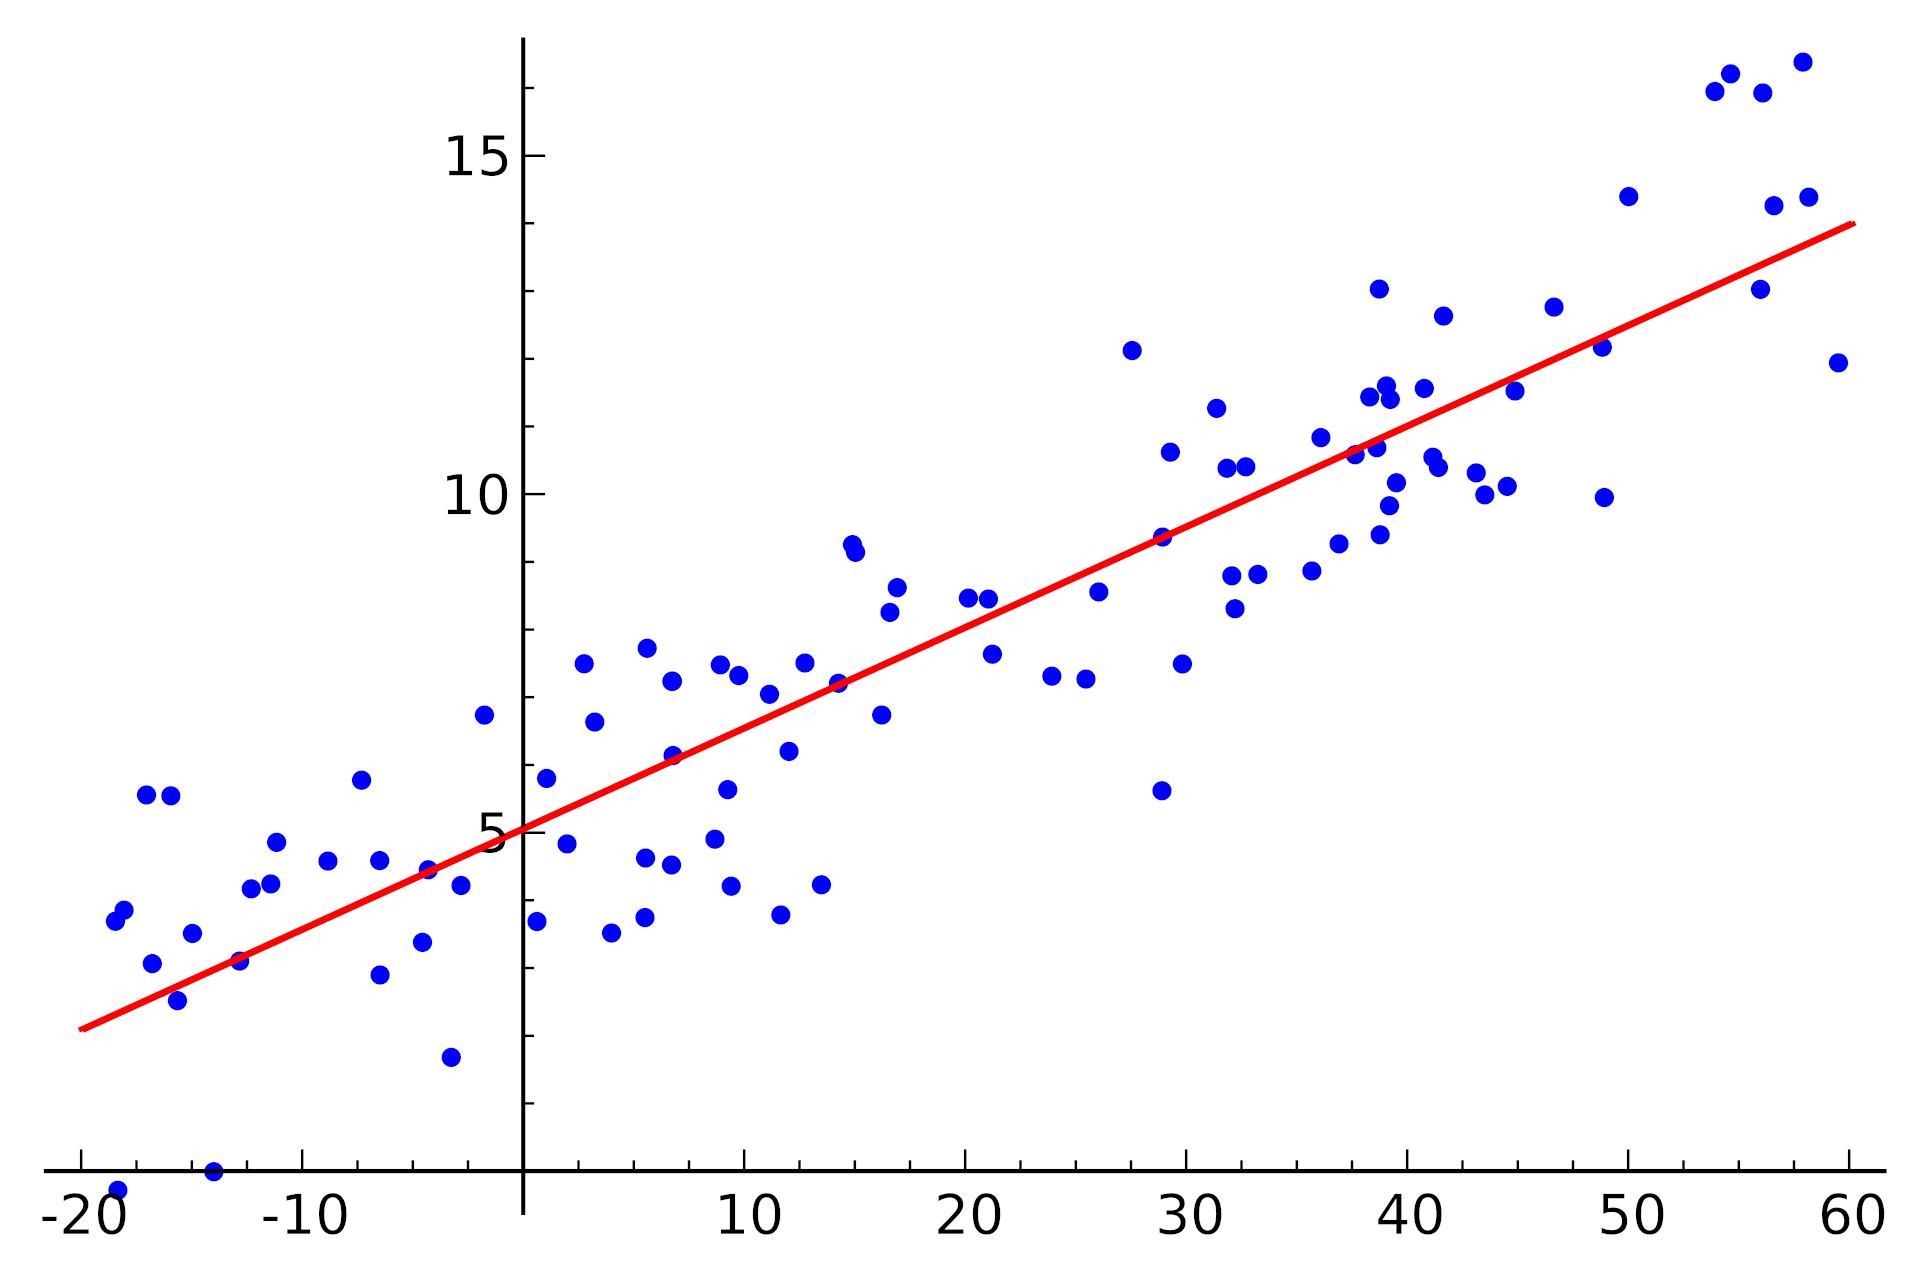
\includegraphics[width=0.6\textwidth]{img/regression_example.png}};
        \end{tikzpicture}

        \pause
        \begin{tikzpicture}[remember picture,overlay]
        \node[xshift=2cm, yshift=-1cm] at (current page.center) {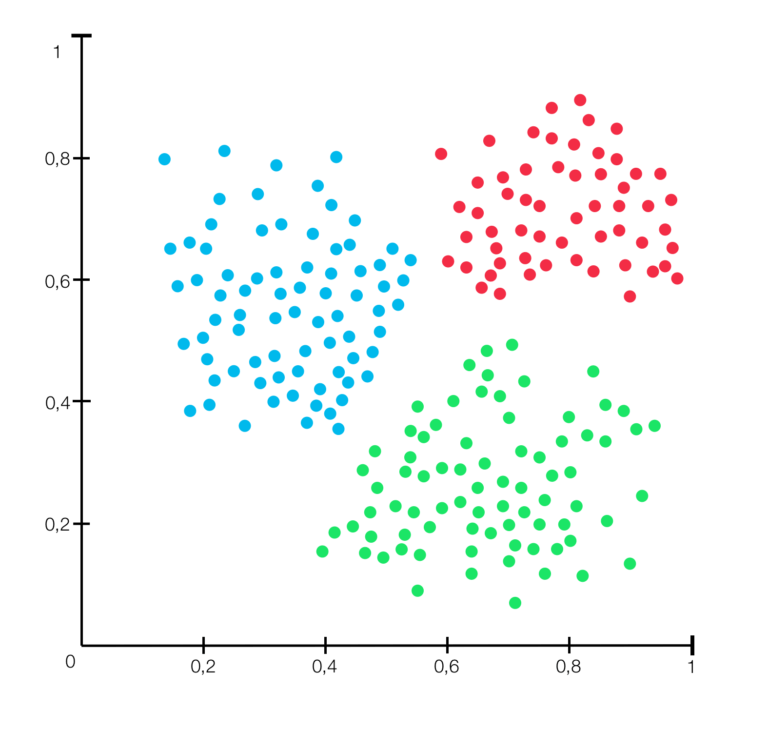
\includegraphics[width=0.5\textwidth]{img/clustering_example.png}};
        \end{tikzpicture}

        \pause
        \begin{tikzpicture}[remember picture,overlay]
        \node[xshift=-2cm, yshift=0.2cm] at (current page.center) {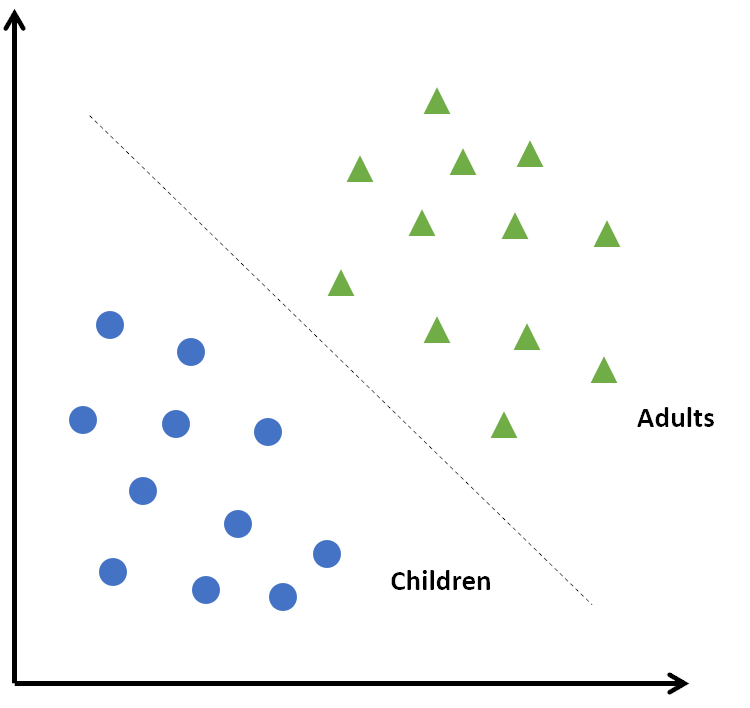
\includegraphics[width=0.45\textwidth]{img/classification_example.png}};
        \end{tikzpicture}

        \pause
        \begin{tikzpicture}[remember picture,overlay]
        \node[xshift=1.2cm, yshift=-0.2cm] at (current page.center) {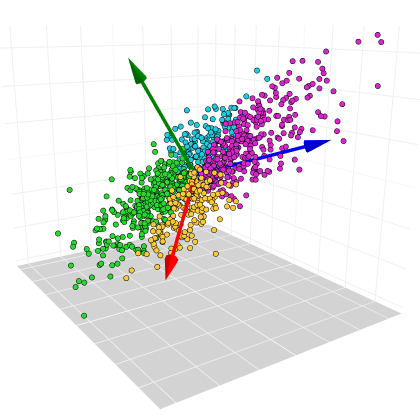
\includegraphics[width=0.5\textwidth]{img/dimensionality_reduction_example.png}};
        \end{tikzpicture}
           
\end{frame}

\begin{frame}
    \vfill
    \begin{itemize}
        \item<1-> ¿Cuál es el problema? ¿Cuál es el objetivo del análisis?
        \item<2-> ¿Qué tipos de variables tengo?
        \item<3-> ¿Cuántos datos tengo?
        \item<4-> \color{black!50!white}¿Tengo muchos outliers? ¿Qué tan robusto debe ser el modelo?
        \item<5-> \color{black!30!white}¿Con cuántos recursos computacionales cuento?
        \item<6-> \color{black!20!white}¿Es importante poder entender cómo el modelo toma decisiones?
    \end{itemize}
\end{frame}

\section{Regresión}

\begin{frame}
    \Huge{Regresión}
    \vspace{0.5em}
    
    \normalsize
    Queremos utilizar los datos que tenemos para poder \textbf{estimar datos que no conocemos} o \textbf{predecir observaciones futuras}. Los valores a predecir son valores \textbf{numéricos}, más precisamente, continuos.

    \vspace{1cm}
    \textbf{Ejemplo:} predecir el valor de un inmueble a partir de su tamaño (m$^2$)
    
\end{frame}

\begin{frame}
    \centering
    \visible<2>{
    \color{red}
    \[
    y = 2x + 50
    \]}\vspace{-0.9cm}
    \begin{overprint}
    \onslide<1>\centering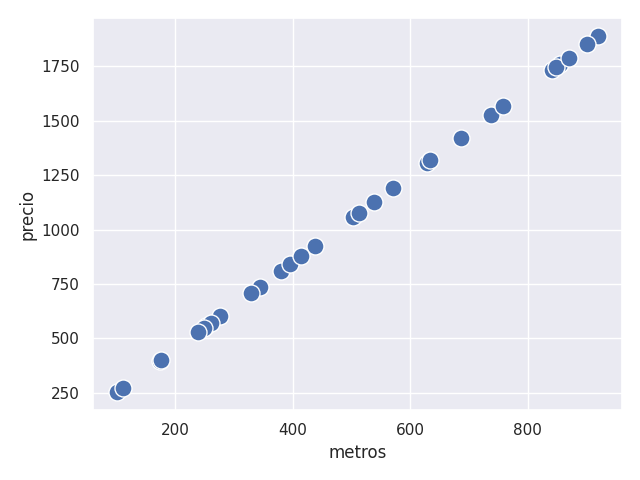
\includegraphics[width=0.65\textwidth]{img/regresion_ej_01.png}
    \onslide<2>\centering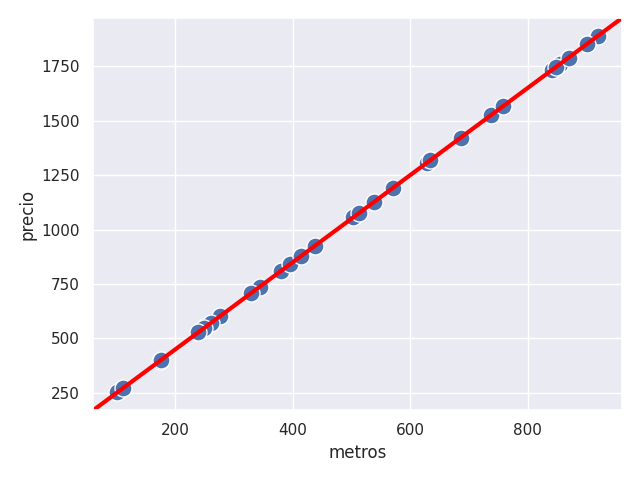
\includegraphics[width=0.65\textwidth]{img/regresion_ej_01_ok.png}
    \end{overprint}  
\end{frame}

\begin{frame}
        \centering
    \visible<2>{
    \color{red}
    \[
    y = 2x + 50
    \]}\vspace{-0.9cm}
    \begin{overprint}
    \onslide<1>\centering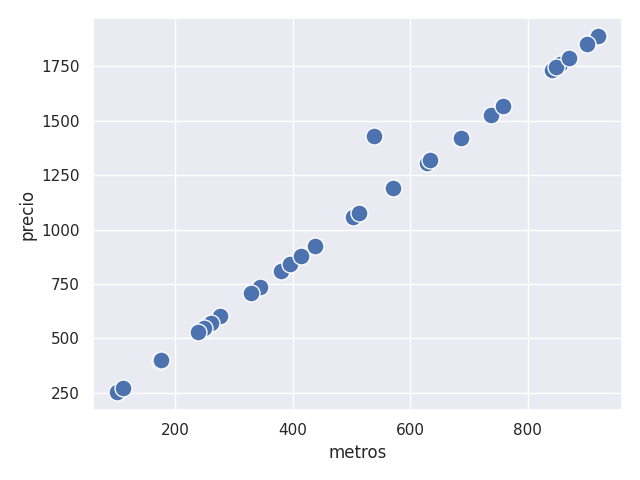
\includegraphics[width=0.65\textwidth]{img/regresion_ej_02.png}
    \onslide<2>\centering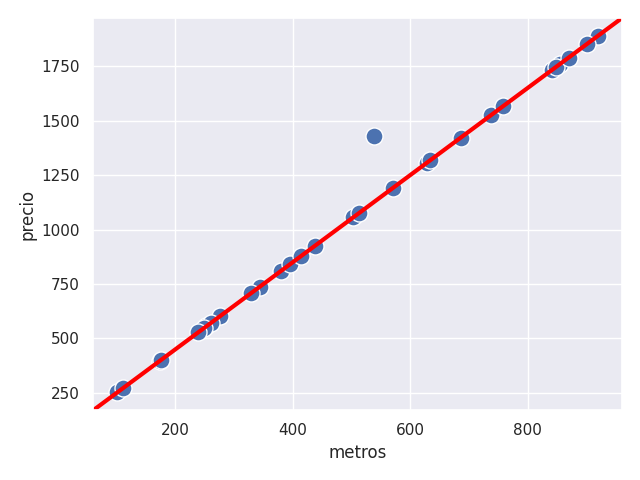
\includegraphics[width=0.65\textwidth]{img/regresion_ej_02_ok.png}
    \end{overprint}  

    \onslide<1>\begin{tikzpicture}[remember picture,overlay]
    \node[xshift=-2.2cm, yshift=0cm] at (current page.east) {
\includegraphics[scale=0.85]{img/meme_01.png}};
    \end{tikzpicture}

    \onslide<2>\begin{tikzpicture}[remember picture,overlay]
    \node[xshift=-2.2cm, yshift=0cm] at (current page.east) {
\includegraphics[scale=0.85]{img/meme_02.png}};
    \end{tikzpicture}
\end{frame}

\begin{frame}
    \centering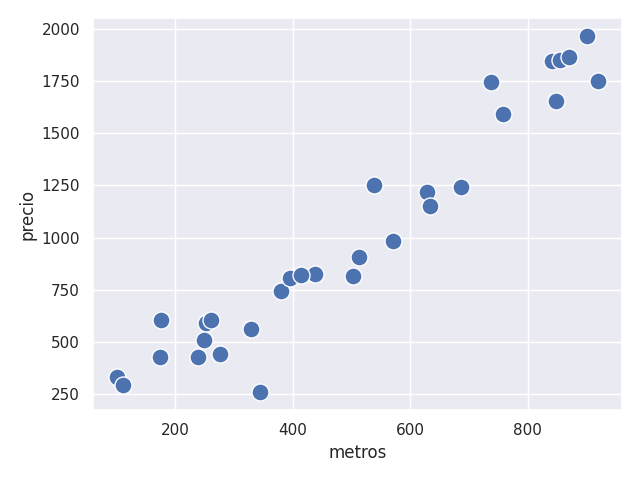
\includegraphics[width=0.65\textwidth]{img/regresion_ej_03.png}

    ¿Qué hacemos ahora?
\end{frame}

\section{Regresión Lineal}

\begin{frame}
        % \fontsize{22pt}{10pt}\selectfont
    \huge
    \[\underbrace{\text{\textbf{Regresión}}}_{\substack{\text{Queremos predecir} \\ \text{un valor continuo}}} {\color{red}\underbrace{\text{ \textbf{Lineal}}}_{\text{con una recta}}}\]
\end{frame}

\begin{frame}
    \textbf{Modelo matemático:} $Y = \beta_0 + \beta_1 X$
    \begin{itemize}
        \item $\beta_0$ es la ordenada al origen
        \item $\beta_1$ es la pendiente
        \item $X$ es la variable predictora
        \item $Y$ es la variable dependiente
    \end{itemize}
    \textbf{Modelo de regresión lineal (simple):} $y_i = \beta_0 + \beta_1x_i + \varepsilon_i$
    \begin{itemize}
        \item $(x_i, y_i)$ son los datos observados
        \item $\varepsilon_i$ es un error aleatorio (variación de $Y$ no explicada por $X$)
        \item $\beta_0$ y $\beta_1$ son \textbf{los parámetros del modelo}
    \end{itemize}
\end{frame}

\begin{frame}
\begin{columns}
    \column{0.4\textwidth}
    \textbf{Residuo:} dados $\beta_0$ y $\beta_1$, definimos al residuo como la diferencia entre el valor observado ($y_i$) y el valor predicho ($\hat{y}_i$):
    \[y_i - \underbrace{(\beta_0 + \beta_1x_i)}_{
     \textstyle \hat{y}_i}\]

    \centering
     \visible<2>{
     \alert{$\rightarrow$ Queremos encontrar valores para $\beta_0$ y $\beta_1$ que \underline{minimicen} los residuos}}
    \column{0.6\textwidth}
    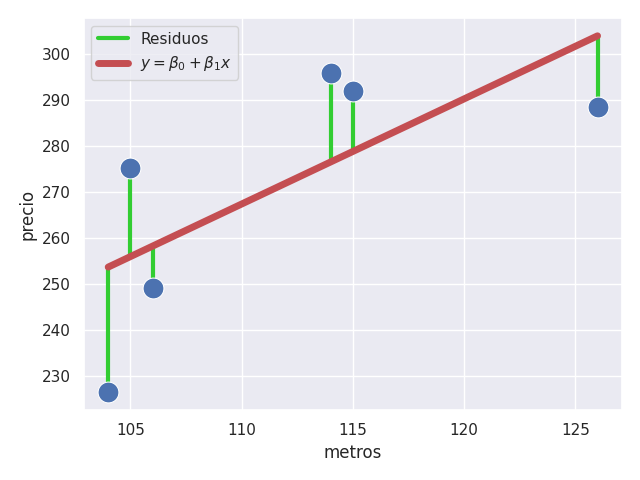
\includegraphics[width=\textwidth]{img/regresion_ej_residuos.png}
\end{columns}
\end{frame}

\begin{frame}
    \Large
    Cuadrados Mínimos
    \vspace{1em}

    \pause
    \normalsize
    Minimizar la suma de los residuos al cuadrado:
    \[
    \begin{array}{rl}
       RSS(\beta_0, \beta_1) =  & (y_1-\hat{y}_1)^2 + (y_2-\hat{y}_2)^2 + \dots + (y_n-\hat{y}_n)^2 = \\
         = & (y_1 - (\beta_0+\beta_1x_1))^2 + \dots + (y_n - (\beta_0+\beta_1x_n))^2 = \\
         = & \displaystyle\sum_{i=1}^n (y_i - (\beta_0+\beta_1x_i))^2
         
    \end{array}
    \]
\end{frame}

\begin{frame}
     Hallamos $\hat{\beta}_0$ y $\hat{\beta}_1$ tales que $\nabla RSS (\hat{\beta}_0, \hat{\beta}_1) = (0, 0)$ :
     \[
     \begin{array}{rl}
          \hat{\beta}_1 = & \dfrac{\displaystyle\sum_{i=1}^n(x_i - \bar{x})(y_i - \bar{y})}{\displaystyle\sum_{i=1}^n(x_i - \bar{x})^2}  \\[1em]
          \hat{\beta}_0 = & \bar{y} - \hat{\beta}_1\bar{x}
     \end{array}
     \]

     donde:
     \[
     \begin{array}{rl}
          \bar{x} =& \dfrac{1}{n} \displaystyle\sum_{i=1}^n x_i  \\
          \bar{y} =& \dfrac{1}{n} \displaystyle\sum_{i=1}^n y_i
     \end{array}
     \]
\end{frame}

\begin{frame}
    \Large
    ¿Qué tan bien ajusta el modelo?
    \vspace{1em}

    \normalsize
    \textbf{Error cuadrático medio (ECM):} cuantifica qué tan cerca está un valor predicho del valor real:
    \[\dfrac{1}{n}\sum_{i=1}^n (y_i - \hat{y}_i)^2\]
\end{frame}

\begin{frame}
    \Large
    ¿Qué tan bien ajusta el modelo?
    \vspace{1em}

    \normalsize
    \textbf{Variabilidad del modelo:} 
    \begin{center}
    \begin{tabular}{rll}
        Variabilidad total: & $\sum_{i=1}^n (y_i - \bar{y})^2$ & {\color{black!50!white}($\approx$ Varianza muestral)}\\
        Variabilidad no explicada: & $\sum_{i=1}^n (y_i - \hat{y}_i)^2$ & {\color{black!50!white} (RSS)}\\
        Variabilidad explicada: & $\sum_{i=1}^n (\hat{y}_i - \bar{y})^2$ &
    \end{tabular}
    \end{center} 
    
\end{frame}

\begin{frame}
    \Large
    ¿Qué tan bien ajusta el modelo?
    \vspace{1em}

    \normalsize
    La proporción de la variabilidad de $Y$ explicada por $X$ se puede explicar como:
    \[R^2 = \dfrac{\text{Variabilidad explicada}}{\text{Variabilidad total}} = \dfrac{\sum_{i=1}^n (\hat{y}_i - \bar{y})^2}{\sum_{i=1}^n (y_i - \bar{y})^2}\]

    \pause
    \vspace{1em}
    \textbf{Obs:} $0\leq R^2 \leq 1$

    A mayor $R^2$ más cercanos están los puntos a la recta y, por lo tanto, tiene más poder de predicción.
    
\end{frame}


\end{document}

